\documentclass[10pt, letterpaper]{article}

\usepackage[margin=0.75in, footskip=0.25in]{geometry}
%\usepackage[superscript, biblabel]{cite} % adding superscript cites
\usepackage[colorlinks]{hyperref}
\usepackage[stable]{footmisc}
\usepackage[T1]{fontenc}
\usepackage{abstract}
\usepackage[skip=0.8pt]{caption}
\usepackage{amsmath}
\usepackage{amsfonts}
\usepackage{amssymb}
\usepackage{amsthm}
\usepackage{wrapfig}
\usepackage{graphicx}
\usepackage{csquotes}
\usepackage{authblk}
\usepackage[english]{babel}
\usepackage{booktabs}
\usepackage{color}
\usepackage{xfrac}
\usepackage[
	backend=biber,
	% numeric, apa, mla, chicago-authordate, ieee, nature, chem-acs, science
	style=apa,
	sorting=none
	% autocite=footnote
]{biblatex}

% \usepackage{xeCJK} % japanese characters
% \setCJKmainfont{IPAMincho}
% \setCJKsansfont{IPAGothic}
% \setCJKmonofont{IPAGothic}

\usepackage{indentfirst}
\setlength{\parindent}{2.5em}
% \usepackage{parskip}
\setlength{\parskip}{0.75em}

\graphicspath{ {./images/} }

% https://tex.stackexchange.com/a/85103/225979
% Add links to images
\ifxetex
	\usepackage{letltxmacro}
	\setlength{\XeTeXLinkMargin}{1pt}
	\LetLtxMacro\SavedIncludeGraphics\includegraphics
	\def\includegraphics#1#{% #1 catches optional stuff (star/opt. arg.)
		\IncludeGraphicsAux{#1}
	}
	\newcommand*{\IncludeGraphicsAux}[2]{
		\XeTeXLinkBox{
			\SavedIncludeGraphics#1{#2}
		}
	}
\fi

\addbibresource{document.bib}
\DeclareLabelname[movie]{
	\field{director}
	\field{producer}
	\field{location}
}

\theoremstyle{definition}
\newtheorem{definition}{Definition}[section]

\definecolor{blue}{rgb}{0,0,0.7}

\hypersetup{
	colorlinks,
	linkcolor=blue,
	filecolor=blue,
	urlcolor=blue,
	citecolor=blue
}

% Remove abstract title
% babel needs \captionenglish
\addto{\captionsenglish}{\renewcommand{\abstractname}{}}
\renewcommand{\absnamepos}{empty}
% Or rename
% \addto{\captionsenglish}{\renewcommand{\abstractname}{New Abstract Title}}

\title{
	% title
	% class name; assignment number; assignment name
	\vspace{-2em}
	Historical Archetypes and Mythology - 1.4 - Functions of Myth
	\vspace{3pt}\\
	% subtitle
 	\large Game Development
}

\author{
	Julián A. Avar C. \thanks{
		ID: \texttt{\#0004984424};
		Term: \texttt{C202112-06};
		Class: \texttt{HIS3320-O};
		Email: \texttt{<jaavarcampopiano@student.fullsail.edu>}
	} \authorcr
	Full Sail University
	\vspace{-1em}
}
% \author[*]{} \affil[*]{}
% \date{}

\begin{document}
	\maketitle
	\vspace{-1em}
	
	\begin{abstract}
		\noindent
		Media Piece: \emph{District 9} \autocite{district_9}\\
		Function of Myth: Sociological
	\end{abstract}

	\pagenumbering{arabic}
	
	\begin{wrapfigure}{r}{0.26\textwidth}
		\centering
		\href{https://en.wikipedia.org/wiki/District_9}{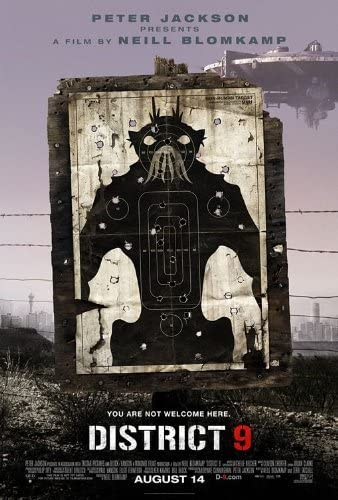
\includegraphics[width=0.26\textwidth]{district_9.jpg}}
		\caption*{\small Theatrical poster for District 9}
		\vspace{-1em}
	\end{wrapfigure}

	The sociological function in mythology is characterized by how it views society in terms of structure; it is a door to ancient society. However and moreover, in modern writing, this tool has multiple uses. (1) In the case that the author is unaware of the societal impact of their piece, or otherwise, of their societal architecture's influence on their piece, then any sociological message that \emph{can} be harvested is not only subtle, but it is also a representation of the culture surrounding the author; their piece serves as anthropological evidence of the culture in which the author stood. (2) In other cases, the author may be less aware, or willing to push a message, simply wanting to indulge in their fantasy. In such cases, the sociological function is no more than ``a subject to pry open'' for the curious eye. (3) This subject becomes more provocative when this tool is used deliberately. The final feature, and one that has been purposefully used --- and overused --- by many authors in modernity, is that in which being aware of the societal structure they (or others) live by, the author chooses to represent it, exaggerate it, or/and contrast it with their own or another. Whether to cause a reaction, root an ideology, or motivate change, it matters little. This cluster of authors is perhaps both the most interesting, and least interesting of any group --- This is where \emph{District 9} finds itself. A story of one of the oppressors who helps the oppressed. And a story we have heard before.
	
	In today's age, such topics relating to societal revolutions are bromidic; from the relatively indirect \emph{Hunger Games} \autocite{hunger_games}, to the more obvious \emph{Bright} \autocite{bright}; many titles, and consequently their authors, are aware of the controversy that stems from structural change and seek reactions from the masses. There are other books and films that draw an even closer comparison still to \emph{District 9}, however, such as \emph{The Last Samurai} \autocite{the_last_samurai}, \emph{Braveheart} \autocite{braveheart}, and of particular interest because of it's thematic similarities and release date: \emph{Avatar} \autocite{avatar}. But we must first understand \emph{District 9} from the most shallow point of view. At face value, \emph{District 9} is a film about the discrimination, xenophobia, and segregation against a group of aliens (which are derogatorily denominated as \emph{``Prawns''}), but is also a very clear allegory to the Apartheid \autocite{apartheid} regime. There is a multitude of factors that contribute to our understanding of the influences, most important of which are the films setting in South Africa, the clear segregation of the Prawns and humans, and the ghetto-like conditions that the Prawns are forced upon reminiscent of the events pertaining District Six in Cape Town.
	
	The film follows a pseudo-documentary format which begins with the tale of a spaceship that arrives at Earth in an alternate 1982, Johannesburg, South Africa. Upon a human investigation team scavenges the spacecraft, over a million malnourished prawns are found and put close to the city, which turns into a ghetto after tensions with the humans who believe the aliens to be aggressive filthy blood-sucking lawbreakers. Sequently, turmoil between the citizens of Johannesburg and the aliens, caused the government to hir Multinational United (MNU), a weapons manufacturer, to relocate the prawns. As an important side note, the viewer is informed that Prawns own incredibly powerful weapons that can \emph{only} be used by Prawns due to some genetic properties, and that in the 20 years the aliens have been on Earth, not once have humans been able to use them. This is where our main protagonist, Wikus van de Merwe (the son-in-law of Piet Smit, an MNU executive), starts. He is represented as an incredibly perverse, weak, cowardly, and most of all \emph{common} individual. As the plot commences, Wikus begins transforming into a prawn due to inhaling an alien black liquid repossessed from one of the aliens to be relocated, and is then hunted down, for organ harvesting and scientific research, by MNU. Loosing his job, wife, friends, and humanity, Wikus desperately --- and coincidentally --- contacts a Prawn that was working with the owner of the black liquid (Christopher Johnson), only to find out that he has a way to operate the spacecraft and leave Earth using the black liquid, but more importantly for our protagonist, that this alien may have a way to return him to normal. And so they break into the MNU lab and steal back the black liquid, murdering dozens in the process. Near the end of the film, while being hunted down by the MNU armada, our near-dead protagonist sacrifices himself to save Christopher and his son, letting them leave Earth given that Christopher could potentially find a cure for Wikus.
	
	At face value, this plot follows the: ``a good white male on the side of the oppressor sacrifices himself to help the oppressed''-template. Our director Neill Blomkamp is guilty of many similarly themed films, and this author would dare to say that all of them are. It gets worse when taking the subjects of \emph{District 9} at face value, i.e. through the film, the Prawns are always portrayed as unintelligent, violent, ugly savages, and not just by the humans, but by how the film presents them. So, it is not only: clearly following Hollywood tropes, it is a wicked deformity, that would be morally incorrect to praise. If not for a presumptuous accident.
	
	Our main protagonist is very flawed, he is everything we (as a modern sensible audience) would try to get away from, and he is given no redemption (i.e. he is left in Earth, presumed captive by the documentary footage, but presumed fully transformed into an in-human Prawn from the film's after-scene). Sure, Wikus might have given a final sacrifice near the end, but this was given while inside a robotic humanoid tank which offered him security. Towards the beginning Wikus aborts a multitude of Prawn eggs and jokes around while doing so, towards the end when Christopher reveals that the black liquid cannot be used as the cure and that he must leave Earth to fetch it, Wikus slams him with a shovel and tries to escape (this is done while the entirety of MNU soldiers are rushing to capture them); Wikus is no hero, he shows close to no growth, and he is not even the villain. Regardless of whether this author presumes these character traits to be done by accident, Wikus is shown to be an incredibly human and common character, with more flaws than not, one which will act irrationally, and one that saves his own skin first. He is the representation of the colonists living in an age where colonialism was accepted rather than rejected. Wikus shows the ugliness of colonialism, and pushes the modern more sensible audience away.
	
	This film attempts to represent history, the social structure that was (debatably) until 1991 South Africa before Nelson Mandela assumed presidency. District 9 is an allegory to District Six, it sends the message that the guilty will not be redeemed, Wikus did not choose to be where he is and he would walk the other had he been given the choice now; change is slow and history is to repeat itself. It shows us the most ugly side of us, and to the most optimist, it gives us a guide of what to avoid.
	
	\emph{District 9} supports the present state of affairs in South Africa, and demonizes the past. It is not the epitome of Campbell’s sociological function definition, but more than anything, this films talks about morality and the way our society has not upheld it in the past, telling us how we should proceed as a society from now on: without segregation, xenophobia, racism.
	
	% use \bigskip when there's not enough content to \clearpage
	% \bigskip
	\clearpage

	\pagenumbering{roman}

	% usually called "References"
	\nocite{release_poster}
	\printbibliography

	\tableofcontents
\end{document}
